\section{Spatial prediction of rentals with socio-demographic data}
\label{sec:8_5_spatial analyses}

In this section I show the methodologies used to predict the demand of cars in a neighborhood without using past data as features. In other words, given only socio-demographic data in the neighborhoods, I try to predict the average number of expected rentals at each time bin, and at each neighborhood.
This problem is often referred to as a green field or cold start approach. In this case, the operator is interested in knowing what could be the system usage in a new neighborhood (or even a new city) based only on socio-demographic data. Historical data are available from other neighborhoods (or cities), and are used only for training.

%\dt{
Since Vancouver presents a division in 22 neighborhoods which constitute the dataset for the training step, the analyses could suffer from an overfitting problem. To minimize this potential effect, I follow a state-of-the-art approach, namely leave-one-out testing: given a target neighborhood, I consider information from all other neighborhoods for training the learning model, and consider the neighborhood that I left out for validation.
%}

I manually select 83 socio-demographic features that might be related to human mobility.  Here, I only apply the Support Vector Regression and Random Forest Regression models, given that they were the best performing models (aside from neural networks) in the temporal prediction.
I do not consider neural networks since these are known to not work well with a very small training set as in this case.
Additionally, being the RFR an ensemble method, it is known to be resilient to overfitting~\citep{Bishop:2006}.

Considering hyperparameter tuning, for SVR, I try three different kernels (linear, polynomial and RBF), with different combinations of parameters. The best performances are obtained for $\epsilon=0.1$, $C=100$ ($C=10$ for RBF), and $\gamma=\frac{1}{\# features}$ ($\gamma=1$ for RBF). For RFR, I try number of trees ranging from 10 to 100. I show the impact of hyperparameter tuning in the following.
  
\begin{figure}
    \begin{center}  
        \begin{subfigure}{0.65\textwidth}
            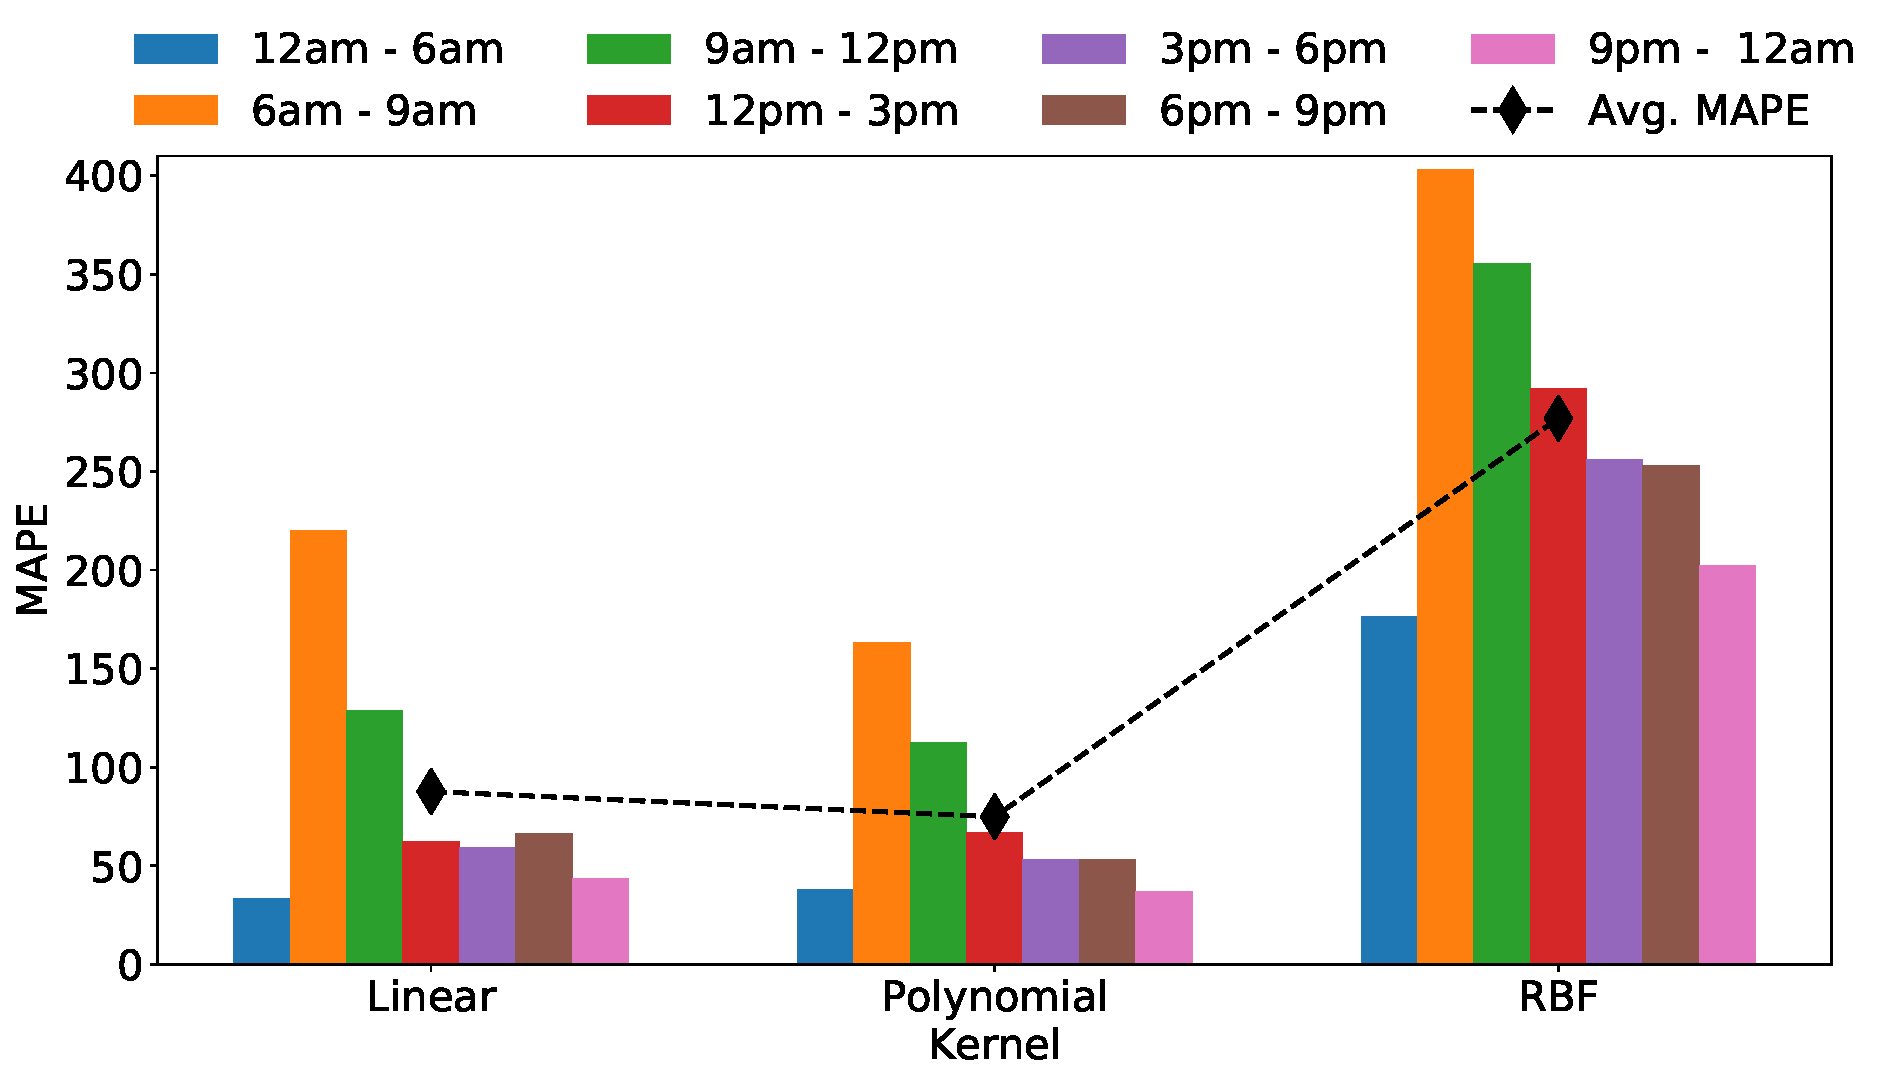
\includegraphics[width=\columnwidth]{figures/spatial_analyses/MAE_hist_svr_start_err_mean_perc.pdf}
            \caption{SVR Model: Starting rentals
            \vspace{0.5cm}}
            \label{fig:8_5_svr_start_MAPE}
        \end{subfigure}
         \begin{subfigure}{0.65\textwidth}
             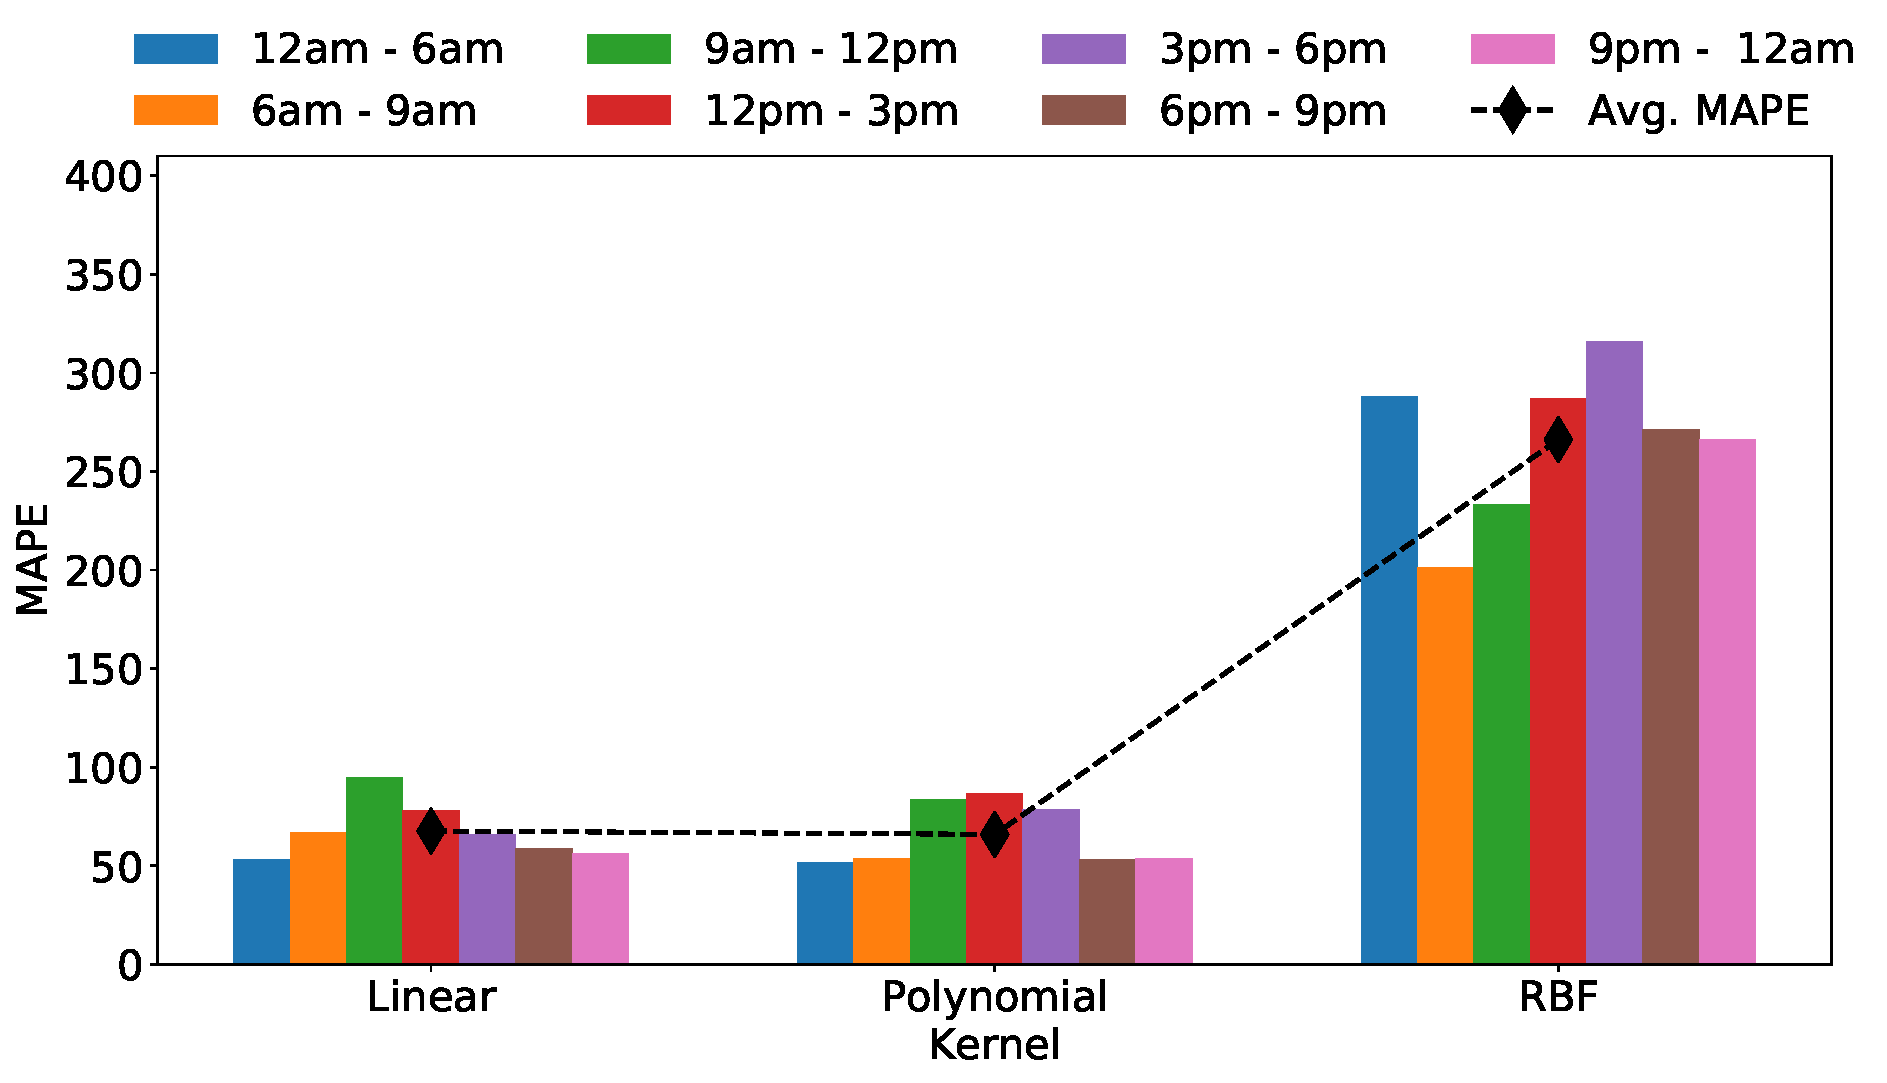
\includegraphics[width=\columnwidth]{figures/spatial_analyses/MAE_hist_svr_final_err_mean_perc.pdf}
             \caption{SVR Model:  Ending rentals}
             \label{fig:8_5_svr_final_MAPE}
         \end{subfigure}
 	\caption{Spatial prediction - MAPE for Support Vector Regression models, using different kernels.}
    \label{fig:8_5_reg_MAPE}
    \end{center}
\end{figure}


\begin{figure}
    \begin{center}
         \begin{subfigure}{0.65\textwidth}
             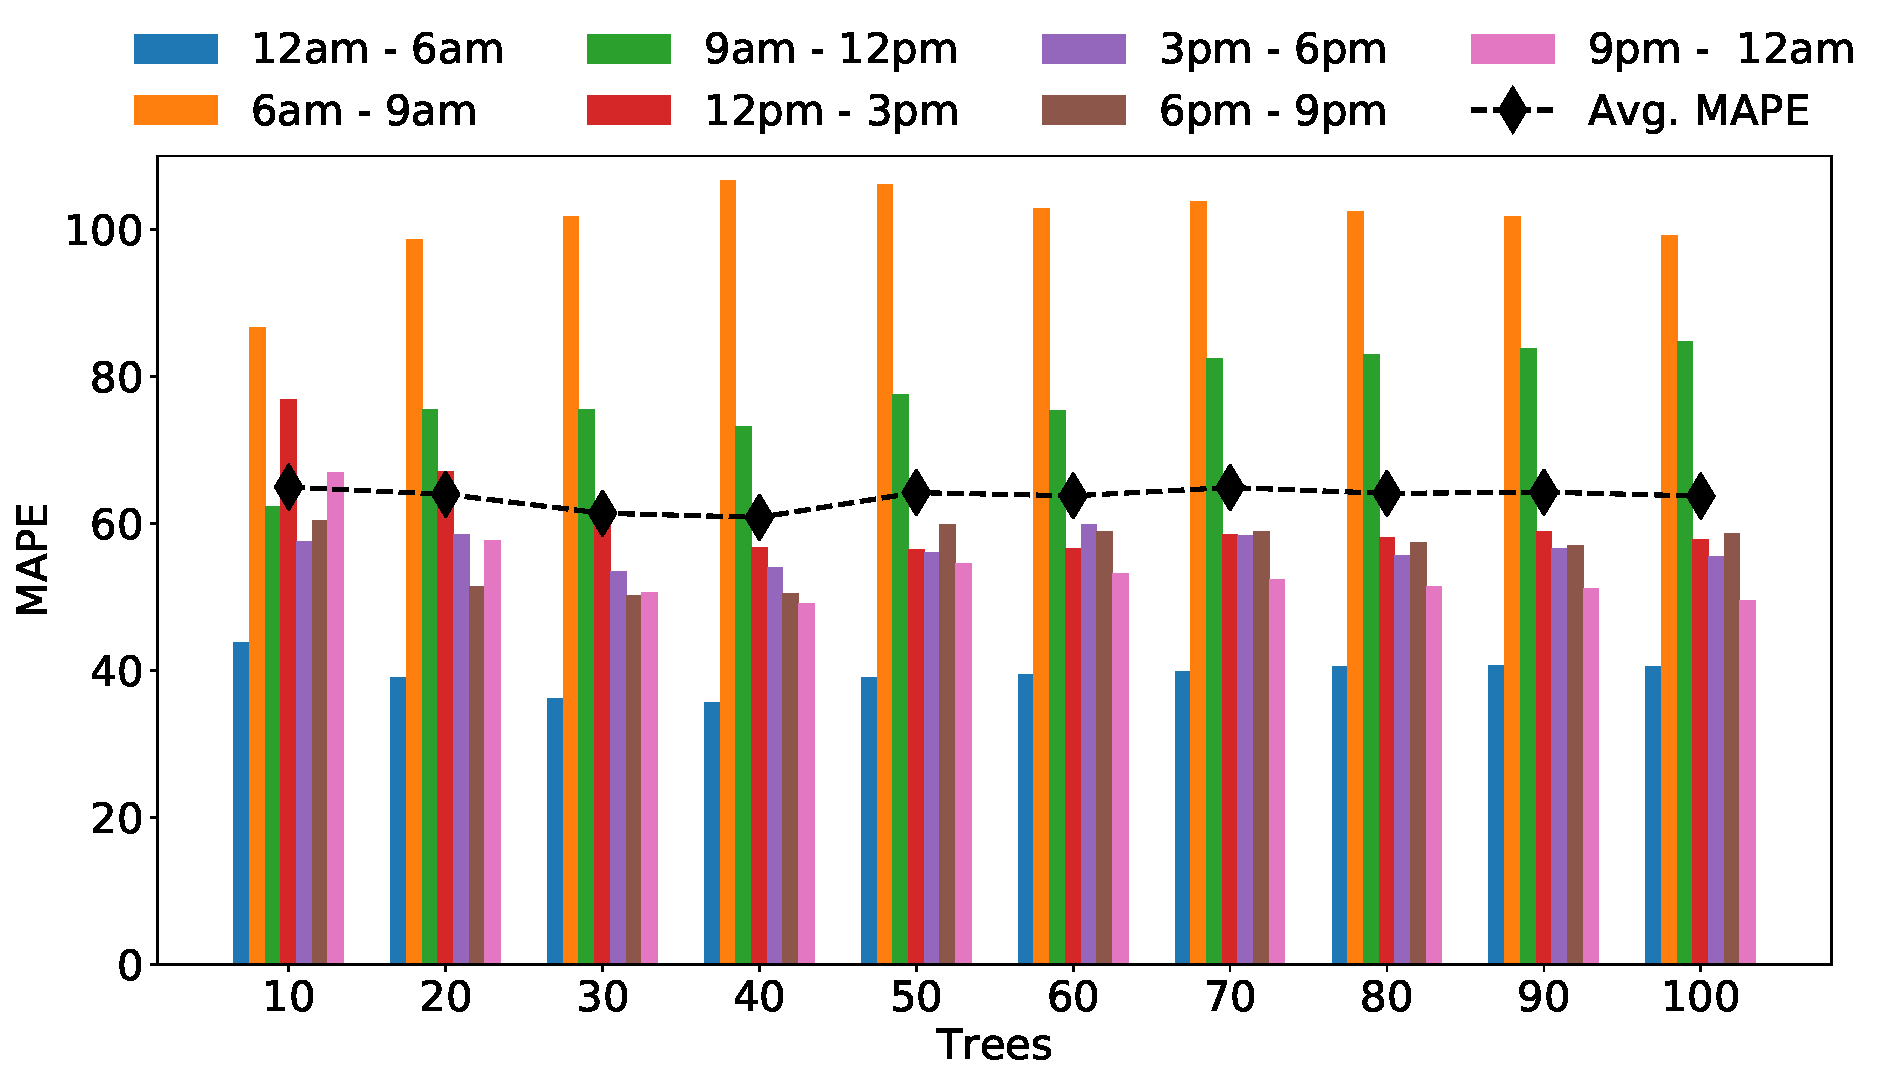
\includegraphics[width=\columnwidth]{figures/spatial_analyses/MAE_hist_rfr_start_err_mean_perc.pdf}
             \caption{RFR Model: Starting Rentals
             \vspace{0.5cm}}
             \label{fig:8_5_rfr_start_MAPE}
         \end{subfigure}
         \begin{subfigure}{0.65\textwidth}
             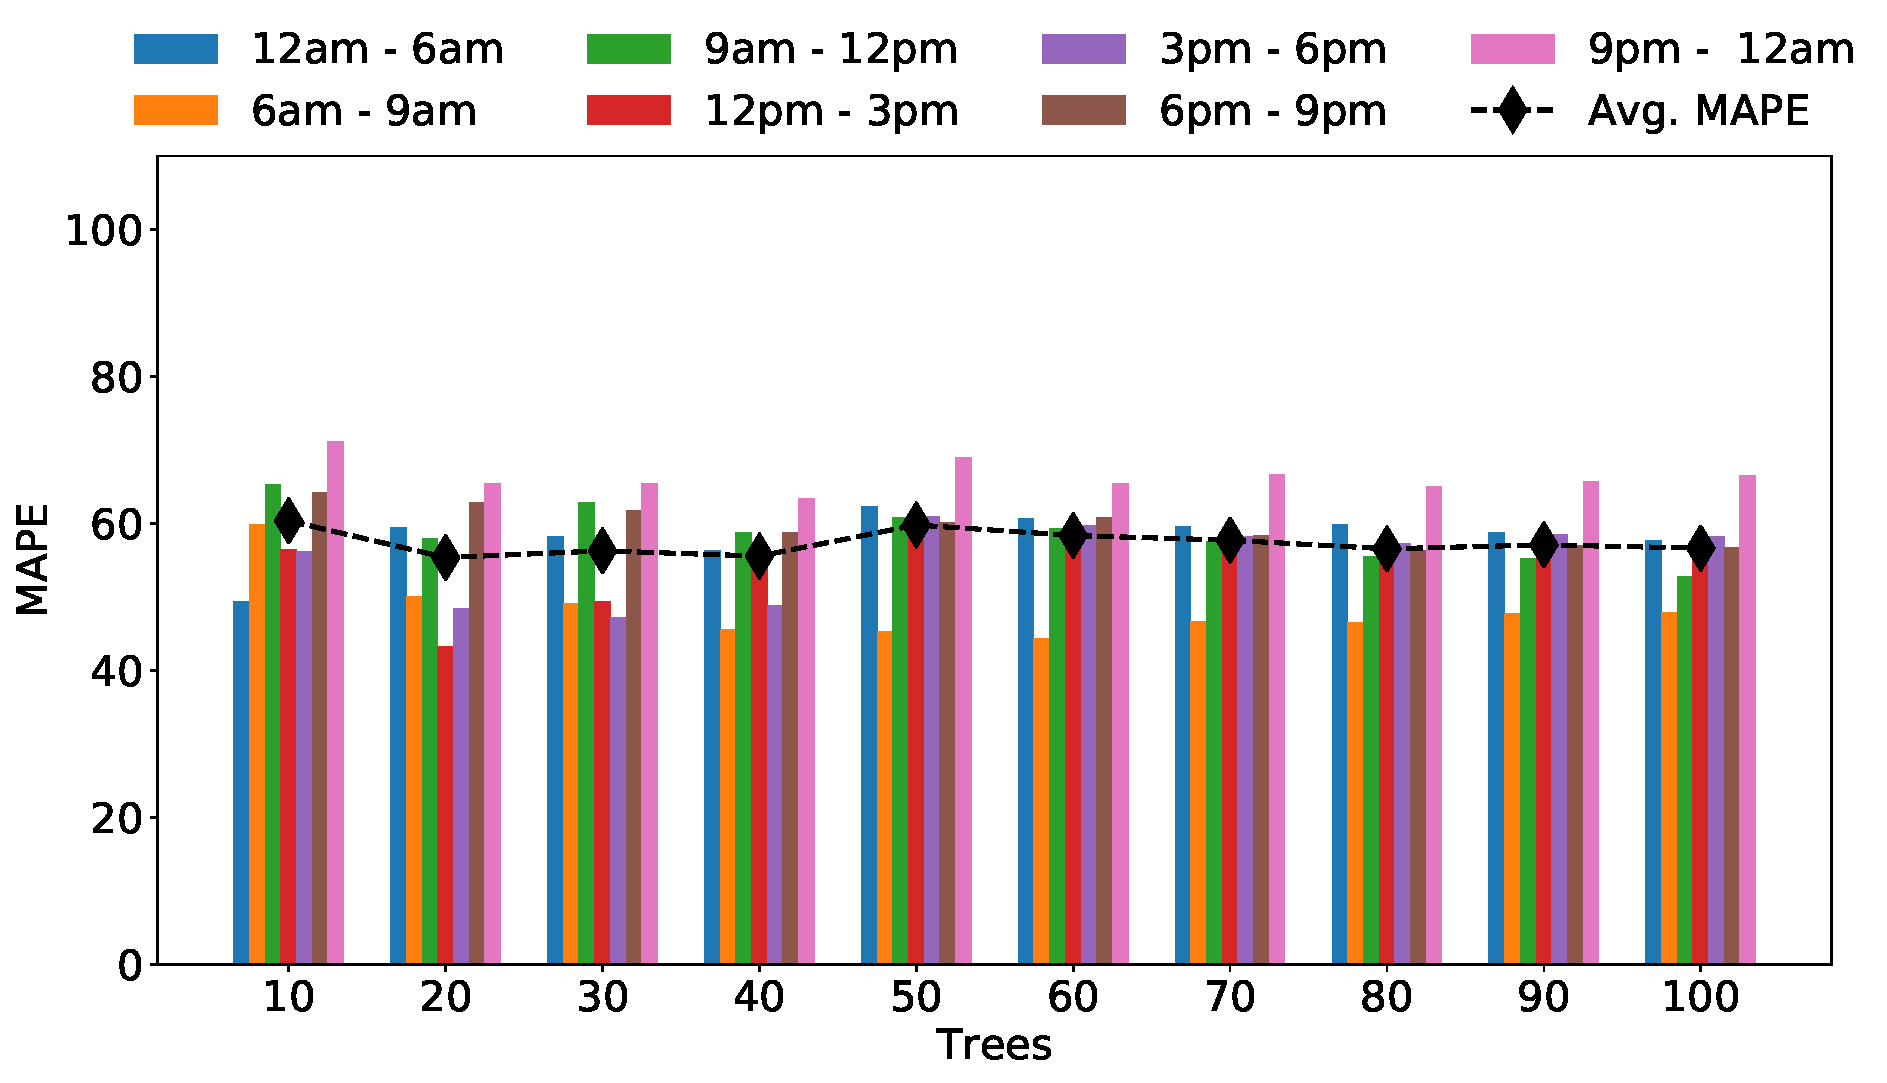
\includegraphics[width=\columnwidth]{figures/spatial_analyses/MAE_hist_rfr_final_err_mean_perc.pdf}
             \caption{RFR Model: Ending Rentals}
             \label{fig:8_5_rfr_final_MAPE}
         \end{subfigure}         
 	\caption{Spatial prediction - MAPE for Random Forests Regression models, using different number of trees.}
    \label{fig:8_5_reg_MAPE_RF}
\end{center}
\end{figure}

Figures \ref{fig:8_5_svr_start_MAPE} and \ref{fig:8_5_rfr_final_MAPE} show the SVR prediction accuracy for the task of predicting the number of starting and ending rentals, respectively. For each kernel type and for each time bin, I report the average MAPE over the 22 experiments (one for each neighborhood that is left out during training). The SVR model performs rather poorly regardless of the parameter setting. Considering the targeted time bin, errors are higher for the morning slots, independently of the kernel, while the time bin from 0\,am to 6\,am is the one for which the model achieves the best performance. The polynomial kernel performs the best: yet the average (over all time bins) MAPE is 70\% for the prediction of starting rentals, and 64\% for the prediction of ending rentals. For the sake of completeness, best RMSE for starting and ending rentals predictions are 499.776 and 427.675, respectively, both for time bin from 0\,am to 6\,am.


The results for the Random Forest Regression model are shown in figures~\ref{fig:8_5_rfr_start_MAPE} and  \ref{fig:8_5_rfr_final_MAPE}, for different number of trees. For a given time bin, I observe limited variation in the MAPE for increasing number of trees, which suggests that a small number of trees (30 or 40 trees, for instance) could be enough. This is expected given again the limited number of samples for the training. In this case, the overall MAPE is 59\%.

Moving to the predictions for ending rentals in figure~\ref{fig:8_5_rfr_final_MAPE}, it is possible to observe smaller errors, with the best case with 20 or 40 trees, with the overall MAPE being 56\%. Again, in the time bin from 0\,am to 6\,am I obtain the best predictions while the worst are obtained from 6\,am to 9\,am (for starting rentals prediction).  Regarding RMSE measure, the best value for starting rentals is 427.260 for time from 0\,am to 6\,am and 50 trees, while for final rentals the best RMSE is 732.825 for time bin 6\,am to 9\,am.
%Differently from the starting rentals predictions,  MAPE does not suffer from high fluctuation. %\ana{Again, why ending rentals are easier to predict?}

Overall, the usage of only socio-demographic data as features offers from quite large prediction error. In the following, I show into which features are the most important so to also perform feature selection and possibly improve the model.

\subsection{Feature ranking and selection}

As in the previous section, I analyze the feature ranking for the RFR model. 
Table~\ref{tab:8_5_featuresranking} reports the top-15 most relevant features. 
This feature ranking procedure allows us on the one hand to identify what information the FFCS operator should focus on when considering new neighborhoods of the city in which to implement its service. 
On the other hand, such ranking leads to a reduction of the number of features the model: in this way it is possible to focus only on the most important ones.

To evaluate the impact of the features on the model performance, I train once again the RFR with an increasing number of features, chosen according to the given rank. I fix the number of trees according to the best average MAPE obtained in Figures~\ref{fig:8_5_rfr_start_MAPE} and \ref{fig:8_5_rfr_final_MAPE}: 40 trees for the starting and 20 for the ending rentals prediction. Figure~\ref{fig:reg_err_perc_LC} shows the results. It reports the MAPE versus the number of features in the model.
Notice the U-shaped curve of the average MAPE (dashed black line). Intuitively, too few features worsen the regression performance due to lack of information. Too many features also reduce the performance since the training is more complicated and the model gets confused.

I further evaluate the RFR model by selecting the best number of features (the one that minimizes the average MAPE), which results to selecting the top 7 features in Table~\ref{tab:results-stationary-models}. With this subset, the average MAPE is 41\% and RMSE equals to 1104.501 for starting rentals, while for arrivals
MAPE is 39\% and  RSME is equal to 1010.453.%\ana{Michele, please check the values.}.
As expected, using only the top most important features improves significantly the performance.

Finally, I explore the spatial prediction error, i.e., I look if there are neighborhoods that present significantly higher errors than others.
Figure~\ref{fig:8_5_error_distributiion} depicts the heatmap of the MAPE per neighborhood, averaged over all time bins. The more the area is red the higher the average MAPE is. Each green dot represents actual positions of starting or arrival rentals as recorded in the original trace.
The areas having the highest error are the ones labelled 15, 18, 11 and 0. The neighborhoods 15, 18, and 0 are in the periphery and intersect only partially with the rental area of the FFCS operator. This mismatch confuses the prediction since the model assumes the operative area coincides with the total area of each neighborhood. Thus, the model predicts much higher numbers of rentals (reflecting the whole neighborhood area) than the ones that are actually done (reflecting the restricted operational area). Neighborhood 0 has instead a large presence of parks where clearly the car cannot operate. As such, the features of this area are also not reflecting the entire area, fooling the classifier.

%\dt{
In general, the performance of the spatial predictions is lower when compared to the temporal predictions. This is expected given the nature of the problem, the limited amount of available data, and because the number of rentals varies widely within each neighborhood. However, I would like to emphasize that the results of the spatial prediction are still quite useful: the ranking of the regions in terms of service demand is indeed preserved in the predictions. In other words, the neighborhood with the largest demands, which could be the preferred locations to extend the service, would still be predicted correctly.
%}



\begin{table}
\centering
\begin{tabular}{lll}
\toprule
\textbf{Rank} & \textbf{Feature}&\textbf{Relevance} \\ \midrule
1  & Number of emergency calls       & 0.0717             \\ \hline
2  & Distance from downtown  & 0.0481             \\ \hline
3  & People commuting by walk           & 0.0381    \\ \hline
4  & People commuting within Vancouver      & 0.0342   \\ \hline
5  & People with income between  100\,000 and 149\,999 \$CAD   & 0.0298 \\ \hline
6  & People with income between  60\,000 and 69\,999 \$CAD     & 0.0286       \\ \hline
7  & People legally recognized as couple   & 0.0281             \\ \hline
8  & People with income more than 150\,000 \$CAD & 0.0274             \\ \hline
9  & People divorced  & 0.0261             \\ \hline
10  & People commuting within the same neighborhood & 0.0249    \\ \hline
11 & Couples having more than 3 children   & 0.0239             \\ \hline
12 & People with age between 50 and 54 years & 0.0233             \\ \hline
13 &  Unemployed people   & 0.0231   \\ \hline
14  & People never married  & 0.0217             \\ \hline
15  & People with income between  80\,000 and 89\,999 \$CAD  & 0.0211  \\ 
\bottomrule
\end{tabular}
\caption{Spatial prediction - Most relevant features and their importance for the prediction using Random Forest Regression. The first 7 are the ones that for obtain the best overall model}
\label{tab:8_5_featuresranking}
\end{table}

\begin{figure}
    \begin{center}
         \begin{subfigure}{0.65\textwidth}
             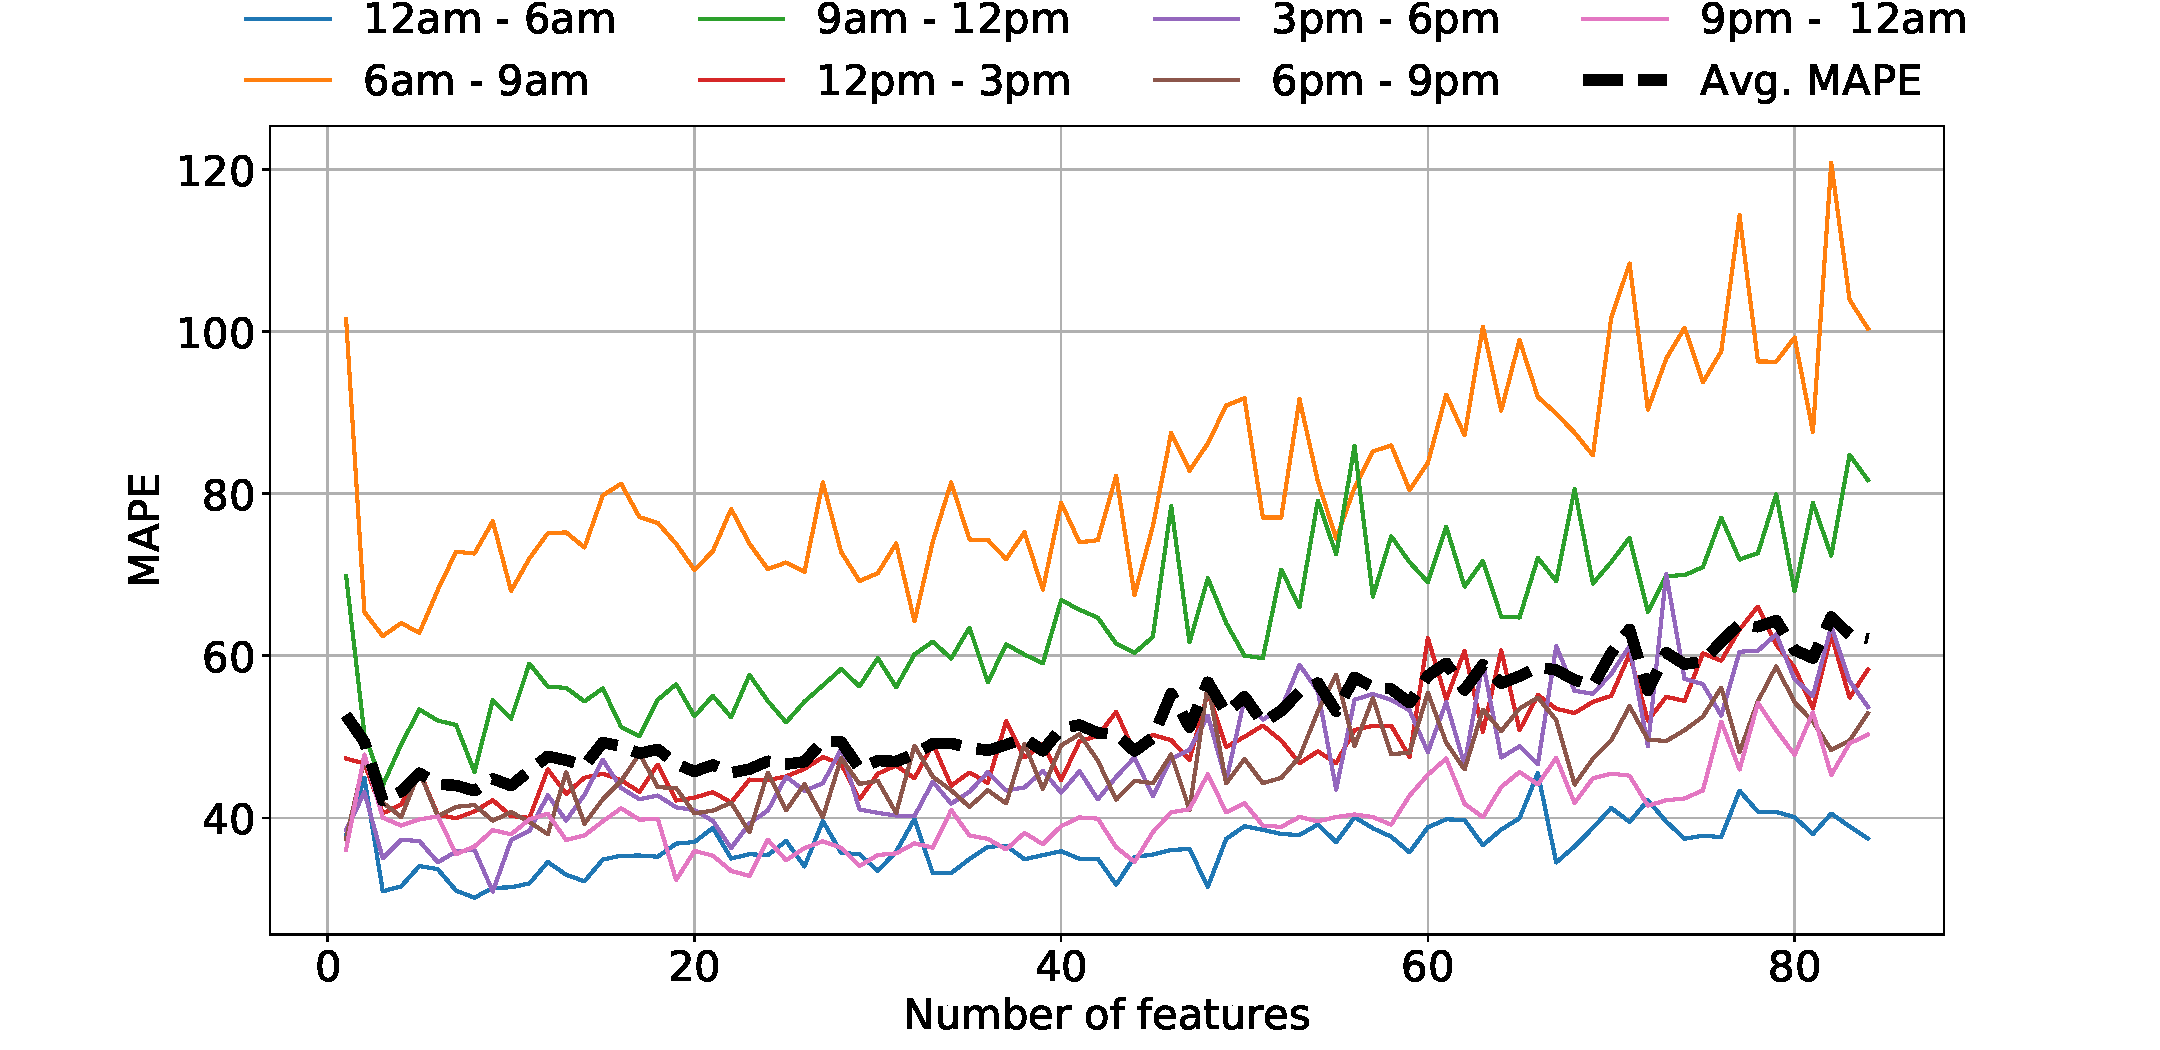
\includegraphics[width=\columnwidth]{figures/spatial_analyses/LC_rfr_True_start.pdf}
             \caption{Rentals starting
             \vspace{0.5cm}}
             \label{fig:8_5_rfr_start_err_lc}
         \end{subfigure}
         \begin{subfigure}{0.65\textwidth}
             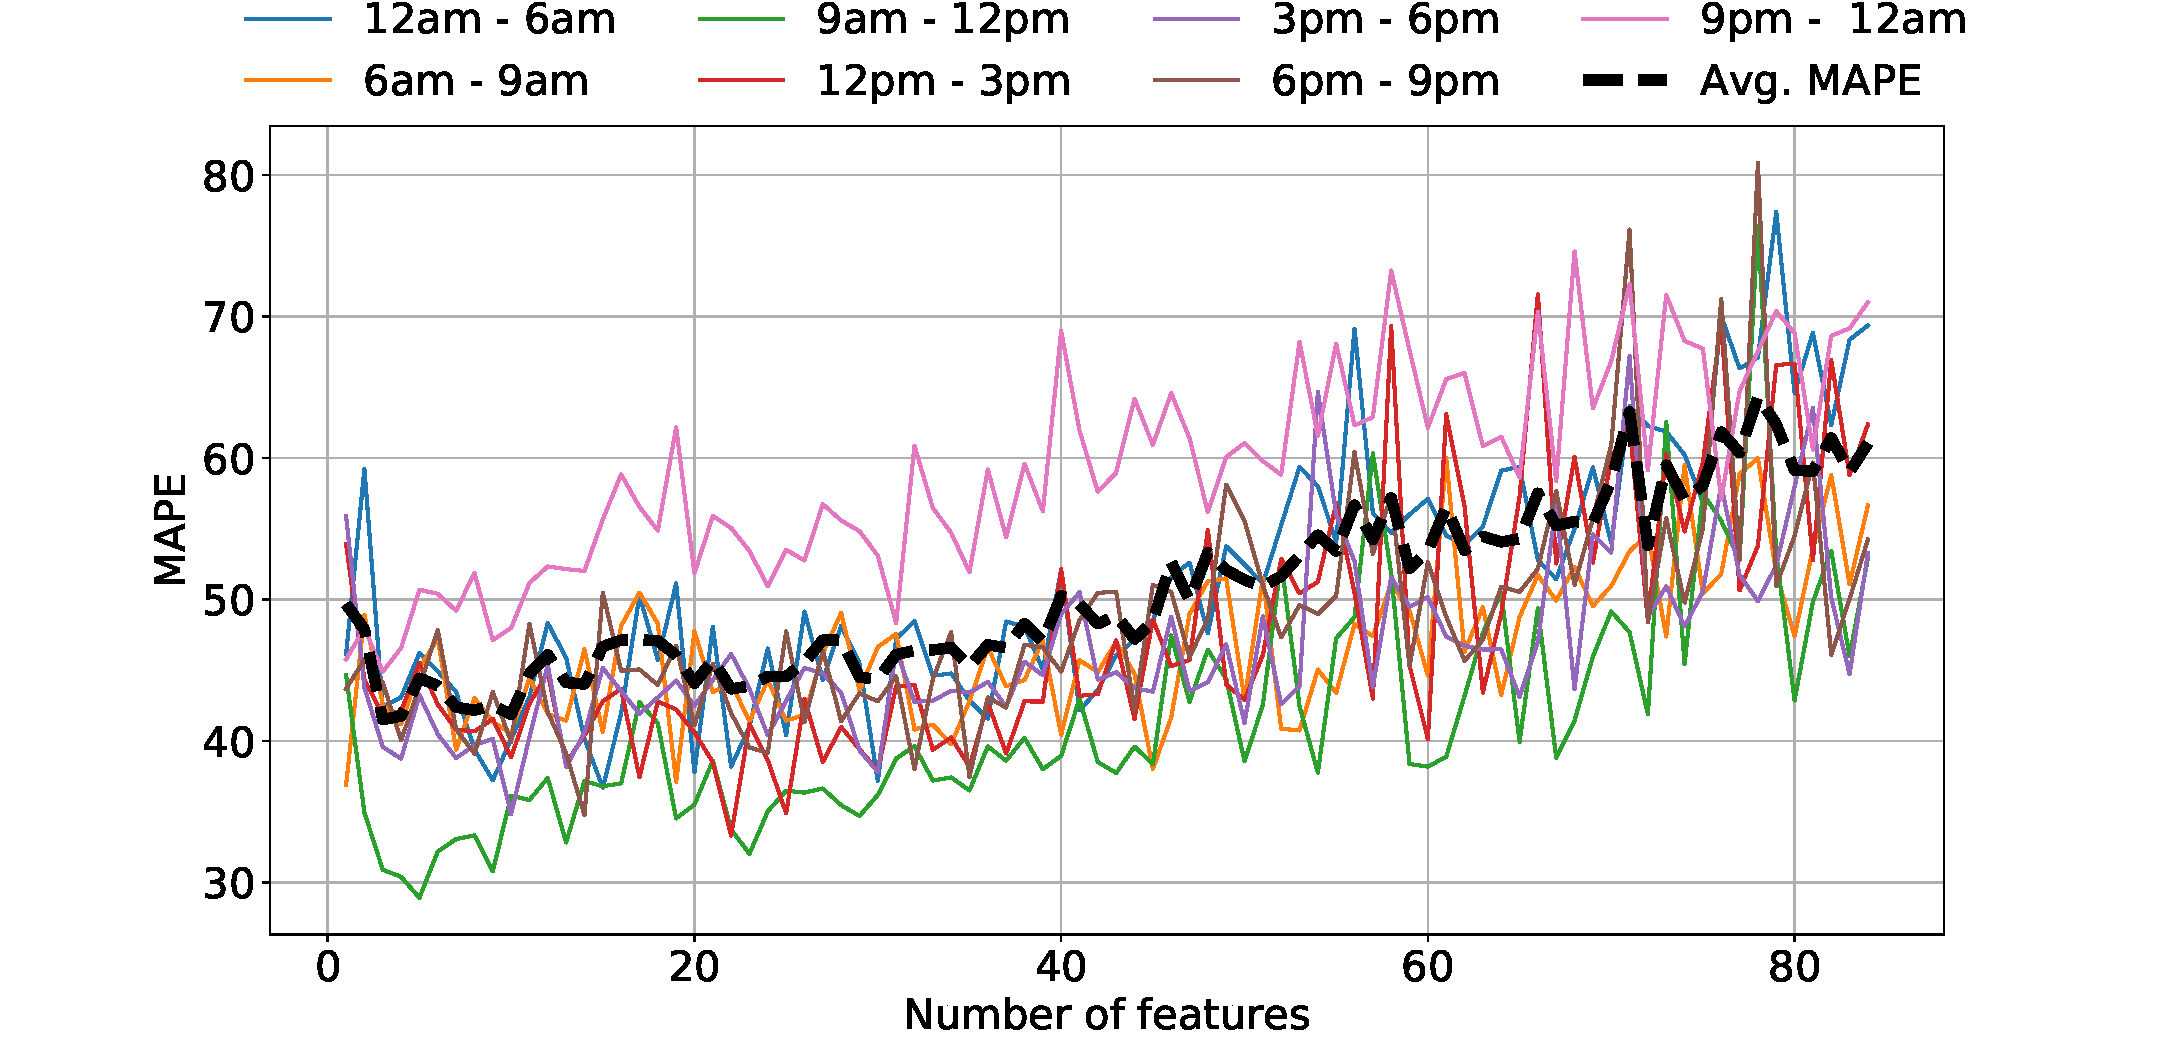
\includegraphics[width=\columnwidth]{figures/spatial_analyses/LC_rfr_True_final.pdf}
             \caption{Rentals arrivals}
             \label{fig:8_5_rfr_final_err_lc}
         \end{subfigure}         
 	\caption{Spatial prediction - MAPE in the different time bins by selecting the most relevant features in RFR}
    \label{fig:8_5_reg_err_perc_LC}
\end{center}
\end{figure}


\begin{figure}
    \begin{center}
        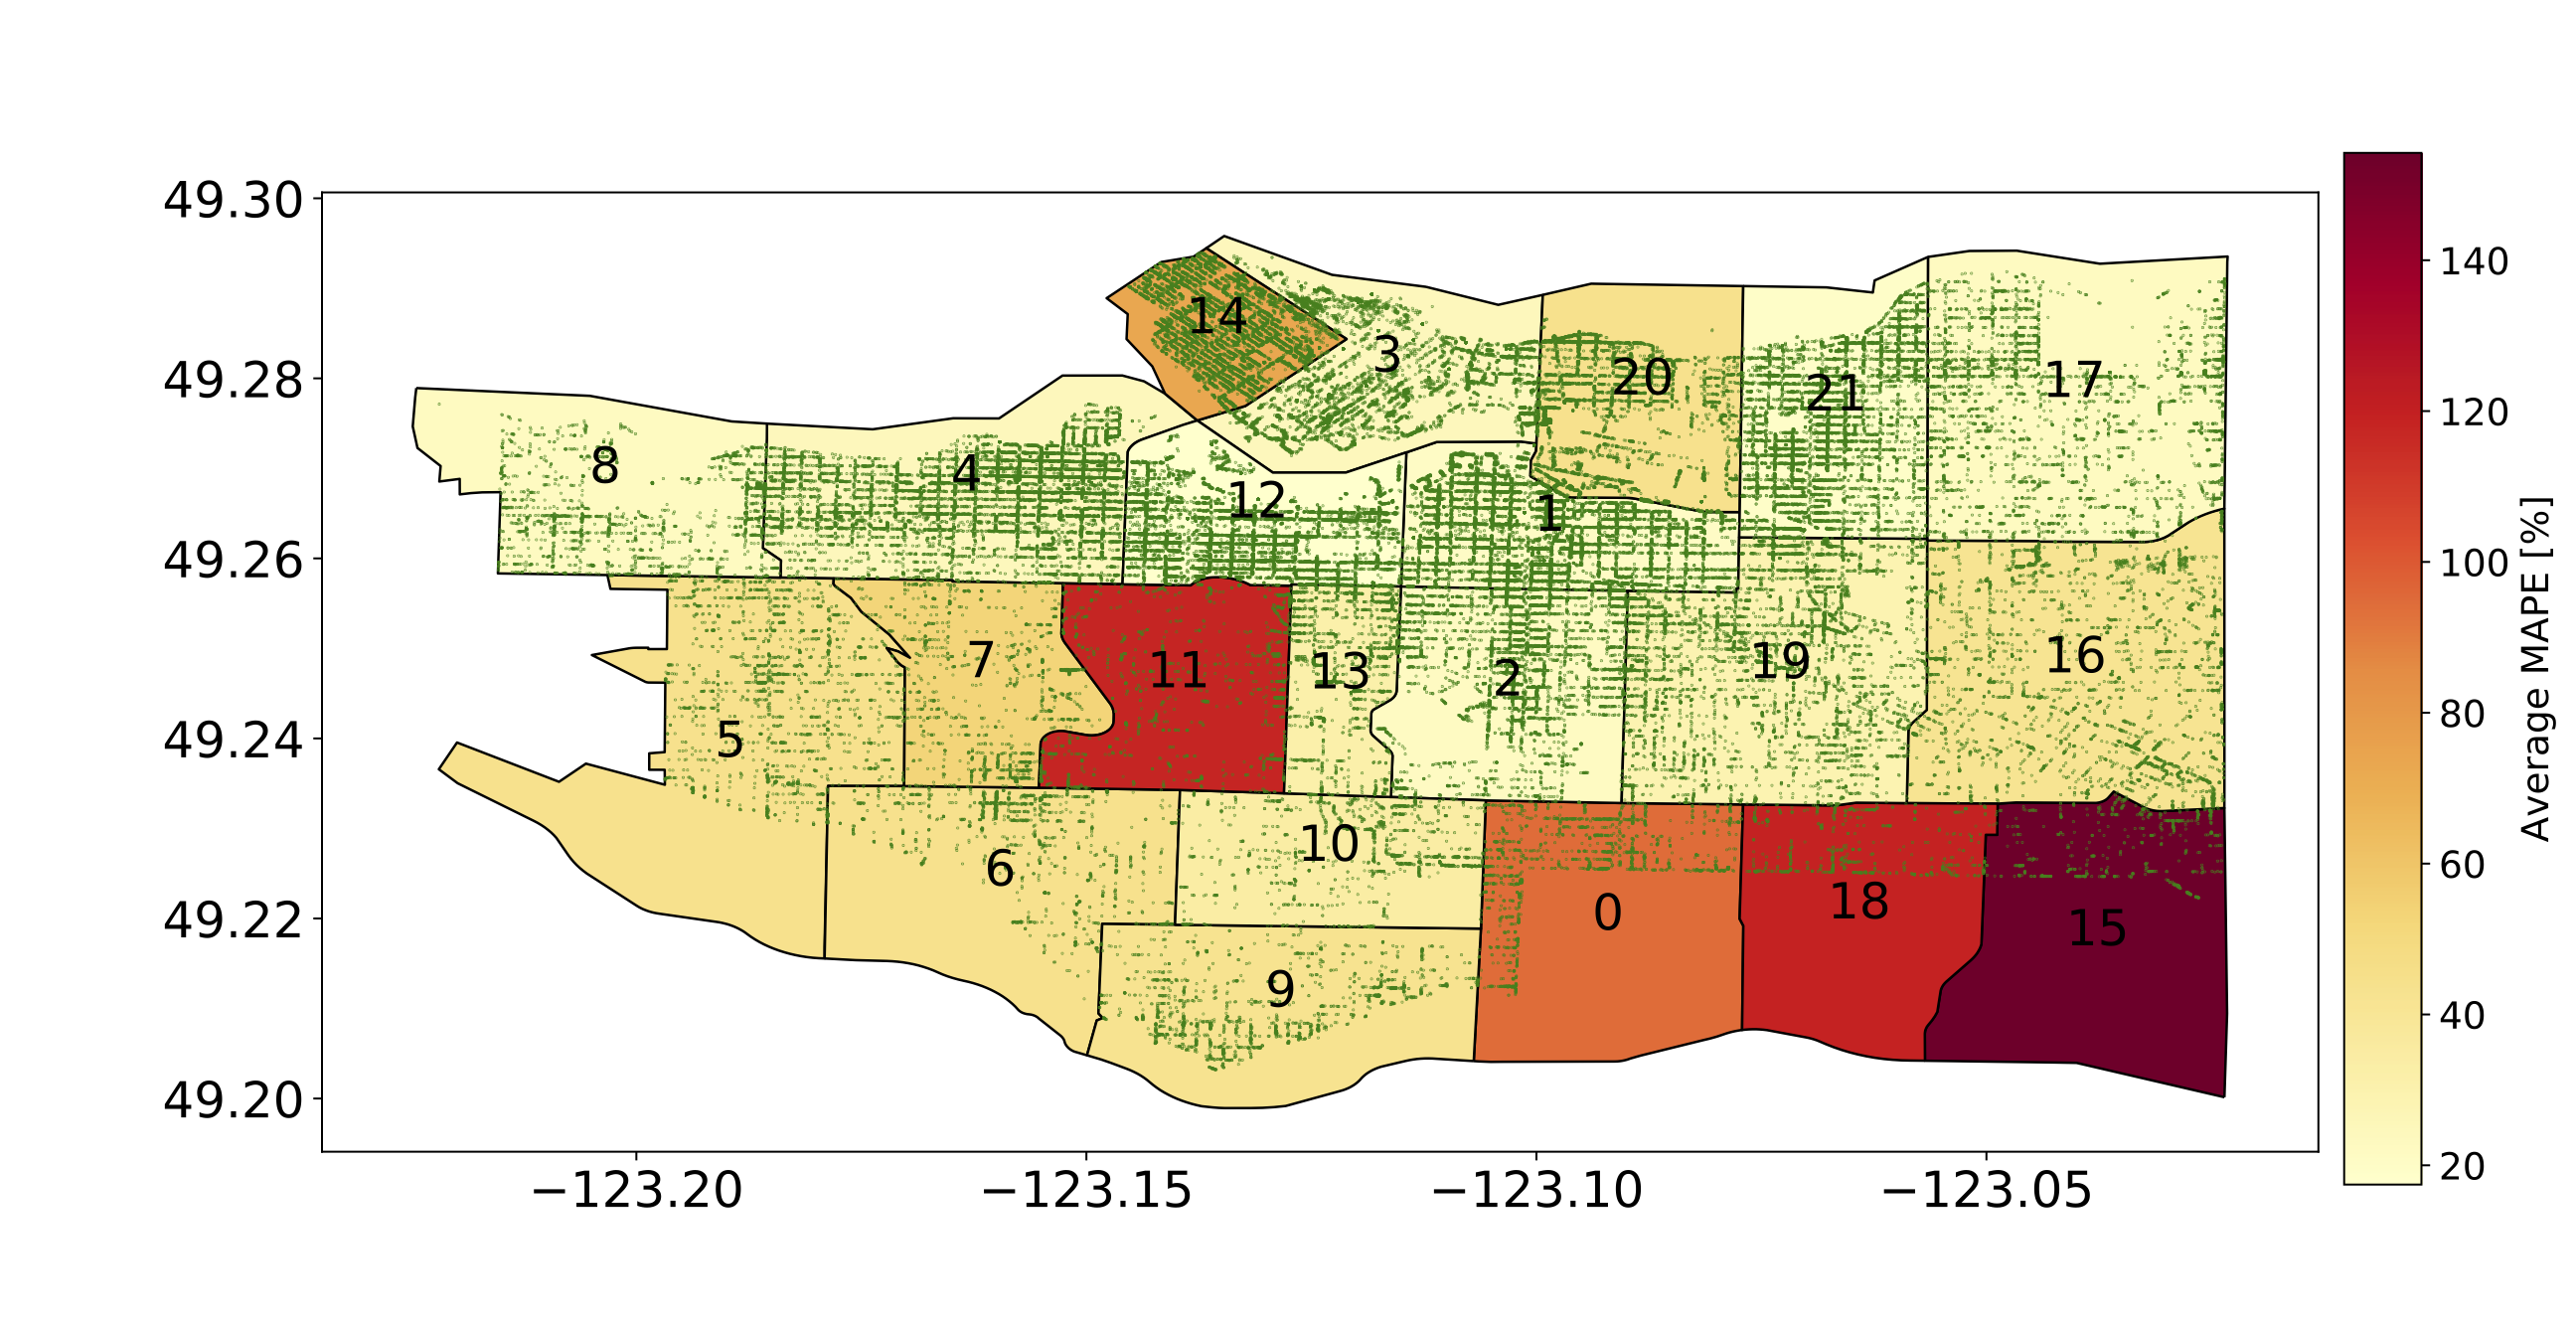
\includegraphics[width=0.7\columnwidth]{figures/spatial_analyses/error_distirbution_map.png}
     	\caption{Spatial distribution - Heatmap of average MAPE per neighborhood. Rentals are shown on the map as green points}
        \label{fig:8_5_error_distributiion}
    \end{center}
\end{figure}